% =====================================================================
%  1bat-ud6-8.tex  —  SESSIÓ 8: L'arbre de l'èxit (diagrames d'arbre i probabilitat total)
%  (sense preàmbul: s'inclou des de main.tex)
% =====================================================================
\horatitol{Sessió 8 — L'arbre de l'èxit (diagrames d'arbre i probabilitat total)}%
{Avaluem un programa d'inserció laboral amb un diagrama d'arbre: calculem la probabilitat global d'èxit i decidim, amb arguments, si val la pena finançar-lo.}

\subsection{Idea clau}

Apliquem els diagrames d'arbre (sessió 7) a l'estudi de cas de l'Activitat 1:
l'\textbf{avaluació d'un programa d'inserció laboral} per a joves. El càlcul de la
\textbf{probabilitat global d'èxit} ens permetrà fer el que fa un tècnic de debò:
\textbf{decidir, amb arguments matemàtics}, si un projecte social és rendible i mereix
recursos públics.

\begin{idea}
\textbf{El cas: un programa d'inserció laboral}
\begin{itemize}[leftmargin=1.4em, itemsep=2pt]
  \item Dels joves que hi entren, el \textbf{$70\%$ supera la formació} (i el $30\%$
        l'abandona).
  \item Dels que \textbf{superen} la formació, el \textbf{$80\%$ troba feina}.
  \item Dels que \textbf{abandonen}, només el \textbf{$30\%$ en troba} pels seus
        mitjans.
\end{itemize}
\textbf{Pregunta:} quina probabilitat té un jove que entra al programa d'acabar trobant
feina? I, amb aquesta xifra, \emph{val la pena} el programa?
\end{idea}

\subsection{Exemples}

\begin{exemple}[l'arbre del programa]
Construïm l'arbre amb les dues etapes (formació $\rightarrow$ feina). Les branques de la
segona etapa són \textbf{condicionades} (depenen de si ha superat o no la formació):

\begin{center}
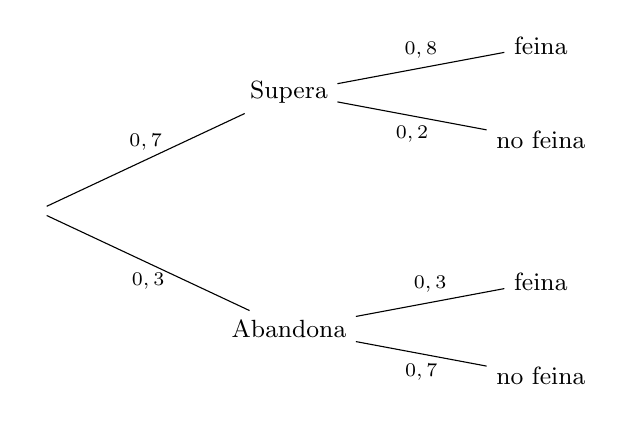
\begin{tikzpicture}[level distance=32mm, sibling distance=9mm,
   every node/.style={font=\small}, grow=right,
   level 1/.style={sibling distance=30mm},
   level 2/.style={sibling distance=12mm}]
\node {} 
  child {node {Abandona}
    child {node {no feina}  edge from parent node[below,font=\scriptsize]{$0,7$}}
    child {node {feina}     edge from parent node[above,font=\scriptsize]{$0,3$}}
    edge from parent node[below,font=\scriptsize]{$0,3$}}
  child {node {Supera}
    child {node {no feina}  edge from parent node[below,font=\scriptsize]{$0,2$}}
    child {node {feina}     edge from parent node[above,font=\scriptsize]{$0,8$}}
    edge from parent node[above,font=\scriptsize]{$0,7$}};
\end{tikzpicture}

\figcap{Les branques de cada node sumen $1$: $0,7+0,3$; $0,8+0,2$; $0,3+0,7$.}
\end{center}

\noindent Hi ha \textbf{dues rutes} que porten a «feina»: superar i trobar-ne, o
abandonar i trobar-ne pel seu compte.
\end{exemple}

\begin{exemple}[la probabilitat global d'èxit]
Multipliquem al llarg de cada ruta i sumem les que porten a «feina»:
\[
P(\text{feina})=\underbrace{0,7\per 0,8}_{\text{supera}}+\underbrace{0,3\per 0,3}_{\text{abandona}}
=0,56+0,09=0,65.
\]
La probabilitat que un jove que entra al programa acabi trobant feina és del
\textbf{$65\%$}. La major part de l'èxit ($0,56$ de $0,65$) ve de la ruta «supera la
formació i troba feina»: el pes del programa està en aconseguir que els joves
\emph{completin} la formació.
\end{exemple}

\subsection{Exercicis resolts}

\begin{exresolt}[interpretar la xifra per decidir]
Amb una probabilitat global d'èxit del $65\%$, és rendible socialment el programa?
Argumenta-ho.
\solucio
Un $65\%$ vol dir que, de cada $100$ joves que hi entren, uns $65$ acaben trobant
feina. Per comparar, cal mirar què passaria \textbf{sense} programa: dels que
abandonen, només un $30\%$ troba feina pel seu compte, de manera que sense la
intervenció l'èxit rondaria el $30\%$. El programa \textbf{més que dobla} la
probabilitat de trobar feina (del $\sim 30\%$ al $65\%$). Amb aquest argument
\textbf{matemàtic}, el programa sembla \textbf{socialment rendible}: la inversió pública
es tradueix en una millora gran i mesurable de la inserció.
\resposta{Sí: passa l'èxit del $\sim 30\%$ (sense programa) al $65\%$ (amb programa);
més que el doble.}
\end{exresolt}

\begin{exresolt}[què passa si millora la retenció]
Si una millora del programa aconseguís que el $90\%$ (en comptes del $70\%$) superés la
formació, quina seria la nova probabilitat global d'èxit? (Mantingues el $80\%$ de feina
dels que superen i el $30\%$ dels que abandonen.)
\solucio
Ara $P(\text{supera})=0,9$ i $P(\text{abandona})=0,1$:
\[
P(\text{feina})=0,9\per 0,8+0,1\per 0,3=0,72+0,03=0,75.
\]
Pujant la retenció del $70\%$ al $90\%$, l'èxit global passa del $65\%$ al
\textbf{$75\%$}. Confirma que \textbf{evitar l'abandonament} és la palanca més potent
del programa.
\resposta{$P(\text{feina})=0,75$ ($75\%$); millorar la retenció apuja molt l'èxit.}
\end{exresolt}

\subsection{Exercicis per fer}

\begin{exercicis}
\begin{exlist}
  \item Amb l'arbre del programa ($70\%$ supera; d'aquests $80\%$ feina; dels que
        abandonen, $30\%$ feina), calcula la probabilitat que un jove
        \textbf{superi la formació i trobi feina} (una sola ruta).
  \item Calcula la probabilitat que un jove \textbf{no} acabi trobant feina (pots
        sumar les dues rutes de «no feina», o fer el contrari de $0,65$).
  \item Un segon programa té: $60\%$ supera la formació; d'aquests, $90\%$ troba feina;
        dels que abandonen, $20\%$. Dibuixa l'arbre i calcula la probabilitat global
        d'èxit. És millor o pitjor que el primer ($65\%$)?
  \item \textbf{(Decisió argumentada)} Amb les dades de l'exercici 3, quin dels dos
        programes finançaries si només en poguessis triar un? Justifica-ho amb les
        probabilitats.
  \item \textbf{(Interpretació)} Al programa original, quina part de l'èxit global
        ($0,65$) ve de la ruta «supera» i quina de la ruta «abandona»? Què et diu això
        sobre on cal posar els esforços?
  \item \textbf{(Raonament)} Per què calcular la probabilitat global d'èxit ajuda a
        \textbf{justificar} una inversió pública en un programa social? Quin avantatge té
        donar una xifra en comptes d'una opinió?
\end{exlist}
\end{exercicis}

% ---------------------------------------------------------------------
\fullsolucions{Sessió 8}
\begin{solucions}
\begin{sollist}
  \item Una sola ruta: $0,7\per 0,8=0,56$ ($56\%$).
  \item Rutes de «no feina»: $0,7\per 0,2=0,14$ i $0,3\per 0,7=0,21$; sumen $0,35$. (O
        bé: $1-0,65=0,35$.) Un $35\%$ no acaba trobant feina.
  \item $P(\text{feina})=0,6\per 0,9+0,4\per 0,2=0,54+0,08=0,62$. És \textbf{una mica
        pitjor} que el primer ($0,62<0,65$).
  \item Resposta oberta. Idea: amb només aquestes dades, finançaria el \textbf{primer}
        programa, perquè té una probabilitat global d'èxit més alta ($0,65$ contra
        $0,62$); a igualtat de cost, dóna més inserció.
  \item Ruta «supera»: $0,56$; ruta «abandona»: $0,09$. La major part de l'èxit ve dels
        que superen la formació, de manera que els esforços s'han de concentrar a
        \textbf{reduir l'abandonament} (que els joves completin la formació).
  \item Resposta oberta. Idea: una probabilitat global és una \textbf{xifra objectiva i
        comparable} que permet contrastar programes, preveure resultats i justificar la
        despesa davant de qui finança; una opinió no es pot comparar ni verificar, però
        un $65\%$ contra un $30\%$ sí.
\end{sollist}
\end{solucions}
